\section{COMPRENSIÓN DEL PROYECTO}
En el presente trabajo se pretende lograr la conducción autónoma básica de un vehículo, al requerir ejecutar pruebas y análisis de resultados, debido a las limitaciones de no contar con el acceso a un vehículo con sensores en la vida real, se hace uso de entorno virtual en un simulador, el elegido para este trabajo es CARLA.

Como primer paso se deben definir los requerimientos, ya que la base de las predicciones son modelos estadísticos basados en datos se tiene la siguiente lista:

\begin{itemize}[nosep]
	\item Módulo de extracción de datos.
	\item Módulo de procesamiento de datos.
	\item Definir las arquitecturas de redes neuronales a utilizar para cada una de las tareas.
	\item Módulo de entrenamiento y evaluación.
	\item Visualización y análisis de las predicciones.
\end{itemize}

Una vez se tengan los datos a disposición, se tiene como objetivo entrenar las redes neuronales en tres tareas de inferencia:

\begin{itemize}[nosep]
	\item Aceleración y giro.
	\item Profundidad.
	\item Segmentación semántica.
\end{itemize}

Utilizando las predicciones de la segmentación para detectar semáforos mediante los contornos, para analizar el color, al igual que las predicciones de distancia para evitar colisiones con otros vehículos.

\begin{figure}[H]
	\centering
	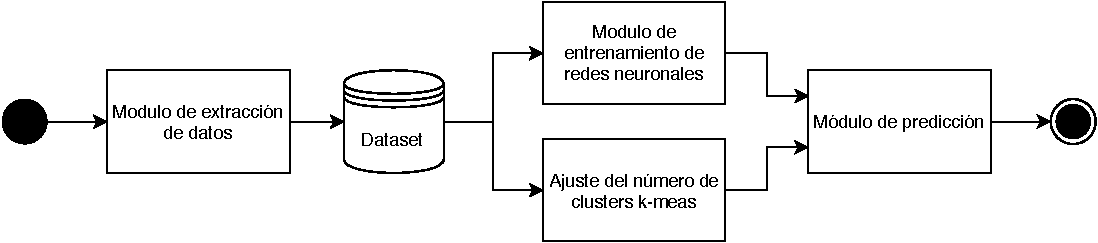
\includegraphics[scale=0.75]{imagenes/arquitectura_proyecto}
	\caption[Arquitectura del proyecto]{arquitectura del proyecto}
	\label{arquitectura_proyecto}
\end{figure}

Así la estructura del proyecto se resume en los componentes descritos en la figura \ref{arquitectura_proyecto}